%%%%%%%%%%%%%%%%%%%%%%%%%%%%%%%%%%%%%%%%%%

\chapter{Testing of components on the West beamline}\label{chap:fall2021}

%%%%%%%%%%%%%%%%%%%%%%%%%%%%%%%%%%%%%%%%%%

In 2021, the ongoing construction of the large \acrshort{msr} (Sec.~\ref{sec:MSR}) relegated the commissioning of nEDM components to the West beamline (Fig.~\ref{fig:AreaB_schematic}).

%%%%%%%%%%%%%%%%%%%%%%%%%%%%%%%%%%%%%%%%%%%%%%

\section{Description of experimental setup (2021)}

%%%%%%%%%%%%%%%%%%%%%%%%%%%%%%%%%%%%%%%%%%%%%%

UCN tau roundhouse. A buffer volume called the ``roundhouse'' was introduced in 2018 that precleans the loaded UCNs and smooths over any temporal fluctuations in the UCN production rate while loading

New Y. NiP coated Vertical separation (center to center of beamline) $\qty{18.85}{in}\approx\qty{0.48}{m}$. Corresponds to a $\sim \qty{25}{neV}$ potential step for upper switcher and a boost to the lower switcher. 

Coils and solenoids (depicted in Fig.~\ref{subfig:west_beamline_switchers}) again keep everything under $\sim \qty{1}{mT}$ field

A second switcher had been constructed for this measurement cycle, was placed on the lower side of the switcher stand. Off this side was the single channel spin analyzer used in Chap.~\ref{chap:north_beamline_paper} and \ref{chap:lanl_ramsey_demonstration}. On the other side was a simultaneous spin analyzer (SSA)

\begin{figure}
\centering
%subfigure width gets "multiplied" by includegraphics width
\begin{subfigure}{.5\textwidth}
  \centering
  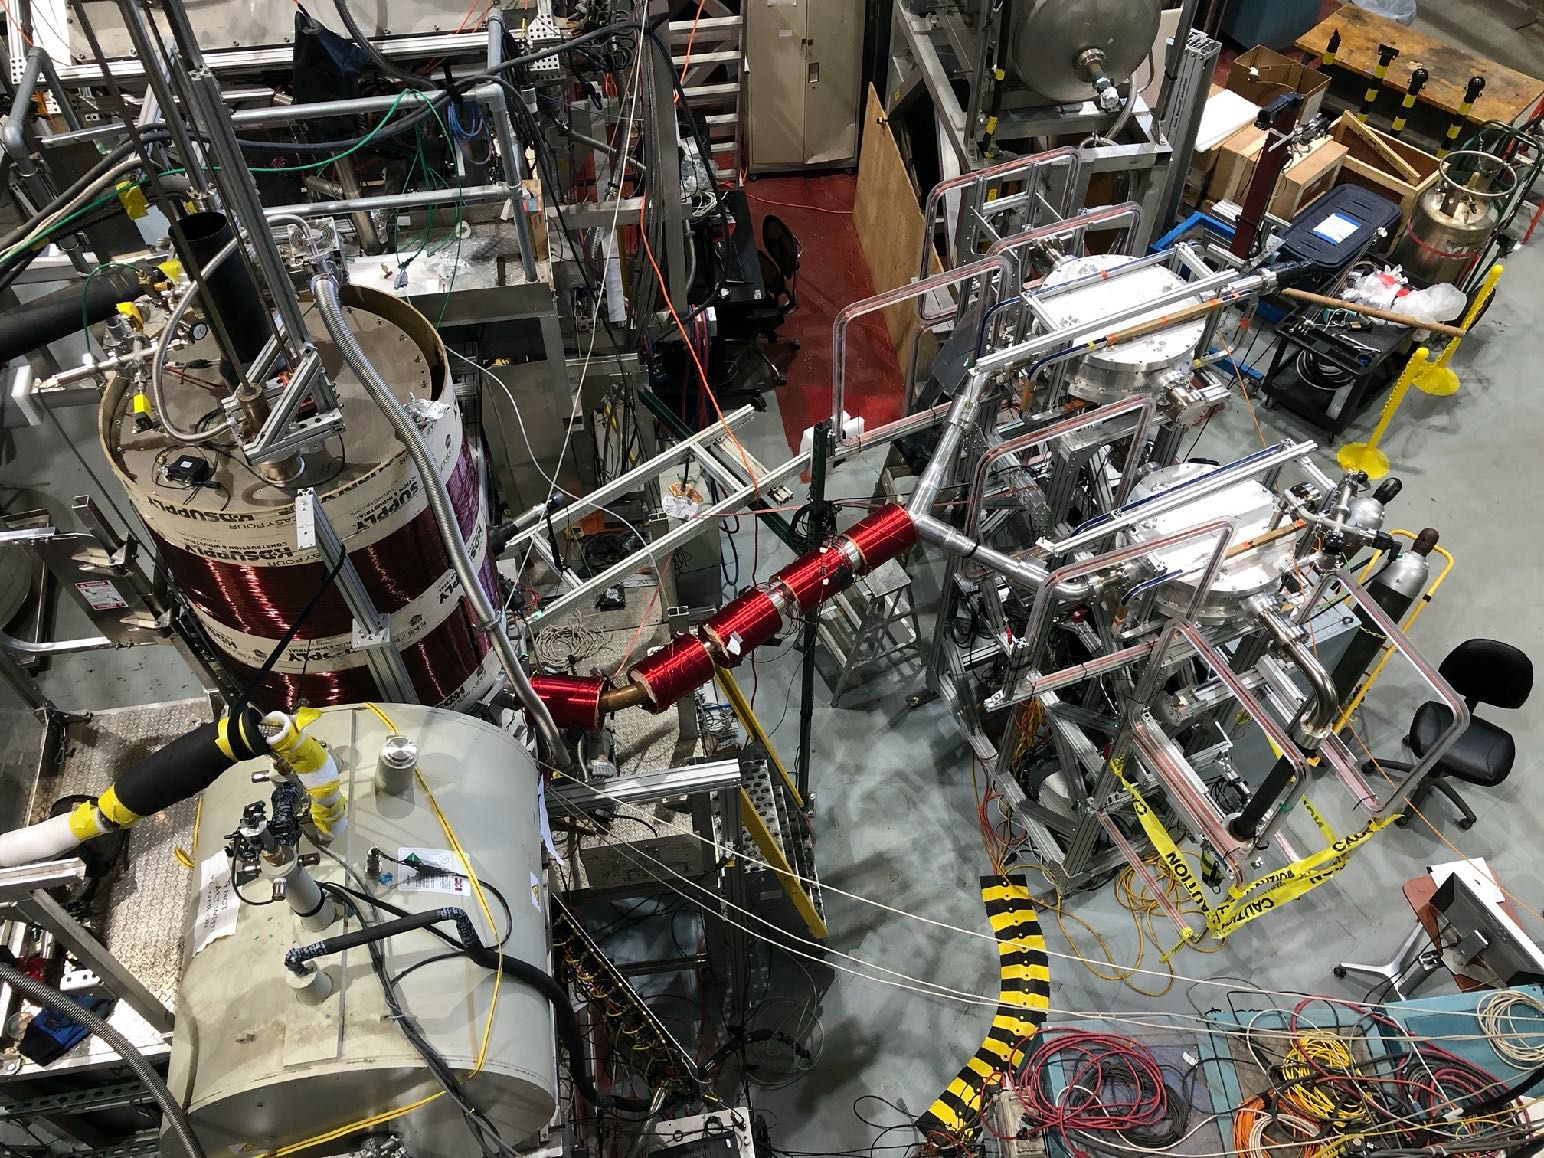
\includegraphics[width=\textwidth]{figures/west_beamline_switcher_tests.jpg}
  \vspace{5pt}
  \caption{}\label{subfig:west_beamline_switchers}
\end{subfigure}%DO NOT REMOVE THIS '%'
\begin{subfigure}{.5\textwidth}
  \centering
  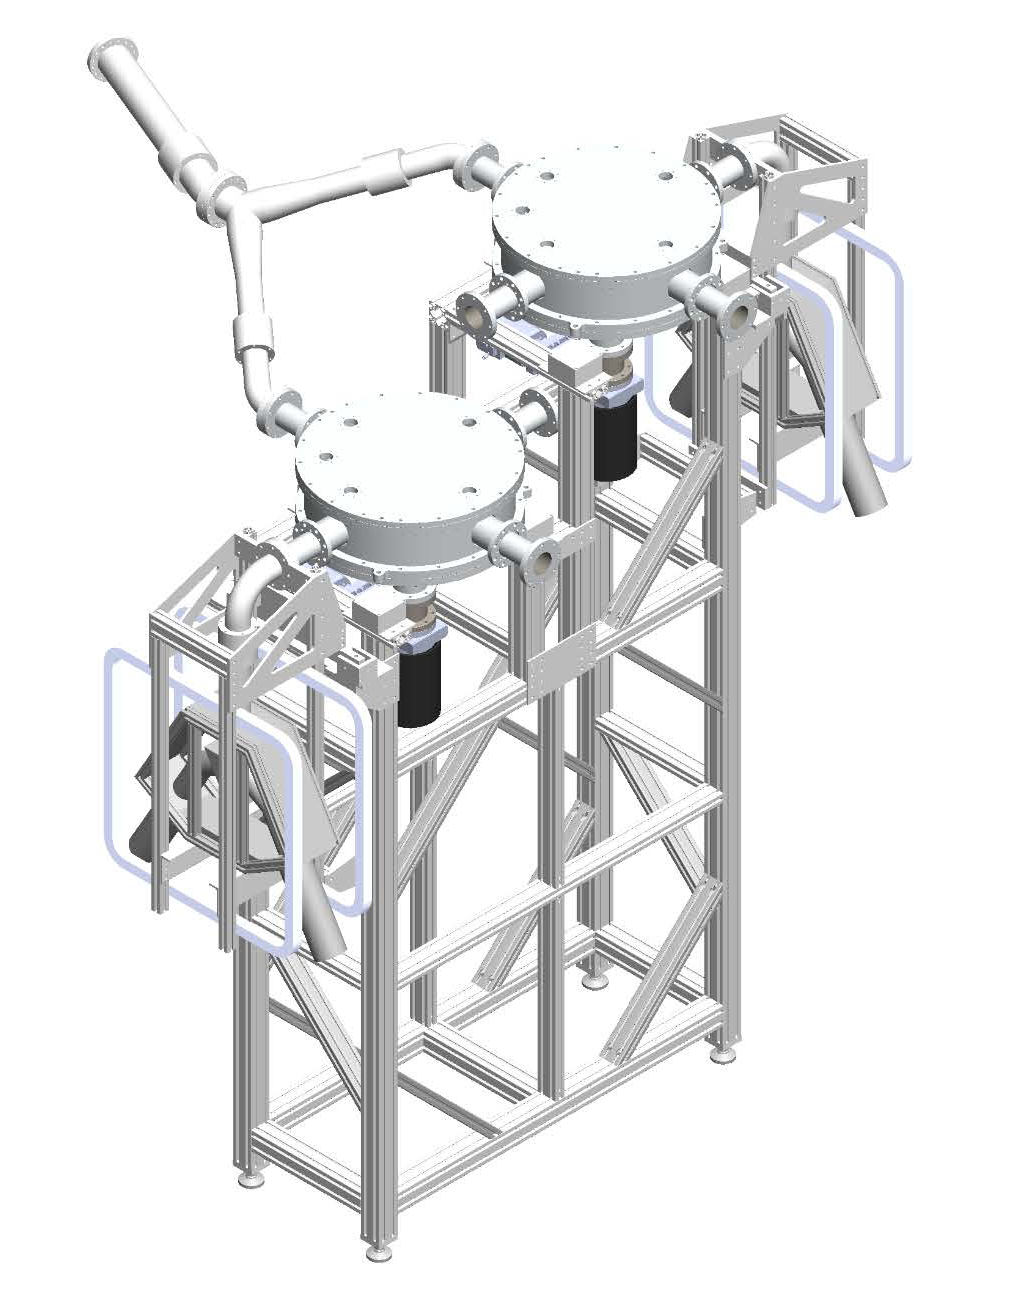
\includegraphics[height=3in]{figures/switcher_mockup.png}
  \caption{}\label{subfig:switcher_mockup}
\end{subfigure}
\caption
{Caption}
\label{fig:west_beamline_switchers}
\end{figure}

%%%%%%%%%%%%%%%%%%%%%%%%%%%%%%%%%%%%%%%%%%%%%%

\section{UCN transport measurements}

%%%%%%%%%%%%%%%%%%%%%%%%%%%%%%%%%%%%%%%%%%%%%%

% Both PMTs beam height on switcher 1 (higher switcher)
% ======================================================
% SINGLE CHANNEL DET FOIL OUT
% detector rate: 1443.88
% wgv rate: 632.46
% normalized to wgv 650 [Hz]: 1483.9230939506056

% BEAM HEIGHT DET: WEST TEST PORT
% detector rate: 1435.18
% wgv rate: 641.26
% normalized to wgv 650 [Hz]: 1454.7406668122135

% BEAM HEIGHT DET: STRAIGHT THROUGH
% detector rate: 1498.215
% wgv rate: 635.39
% normalized to wgv 650 [Hz]: 1532.6645839563103

% Beam height PMTs on both switchers
% ======================================================
% SINGLE CHANNEL DET FOIL OUT
% detector rate: 1465.2666666666667
% wgv rate: 656.6
% normalized to wgv 650 [Hz]: 1450.5381256980404

% BEAM HEIGHT DET: SWITCHER 2 (LOWER)
% detector rate: 2244.225
% wgv rate: 650.0416666666666
% normalized to wgv 650 [Hz]: 2244.0811486443176

% BEAM HEIGHT DET: SWITCHER 1 (HIGHER)
% detector rate: 1512.1142857142856
% wgv rate: 649.5142857142857
% normalized to wgv 650 [Hz]: 1513.2450622443143

% Switcher 2 transmission difference: 1.5425987599300384

%%%%%%%%%%%%%%%%%%%%%%%%%%%%%%%%%%%%%%%%%%%%%%

\section{Simultaneous spin analyzer tests}

%%%%%%%%%%%%%%%%%%%%%%%%%%%%%%%%%%%%%%%%%%%%%%

Led to changes where the RF coil was replaced and shifted higher on the Y. Also 